\documentclass[11pt,journal, a4paper]{IEEEtran}

\makeatletter
\newcommand\subparagraph{%
  \@startsection{subparagraph}{5}
  {\parindent}
  {3.25ex \@plus 1ex \@minus .2ex}
  {-1em}
  {\normalfont\normalsize\bfseries}}
\makeatother
\usepackage{titlesec}
\let\subparagraph\relax % You don't want to use \subparagraph

% some very useful LaTeX packages include:

%\usepackage{cite}      % Written by Donald Arseneau
                        % V1.6 and later of IEEEtran pre-defines the format
                        % of the cite.sty package \cite{} output to follow
                        % that of IEEE. Loading the cite package will
                        % result in citation numbers being automatically
                        % sorted and properly "ranged". i.e.,
                        % [1], [9], [2], [7], [5], [6]
                        % (without using cite.sty)
                        % will become:
                        % [1], [2], [5]--[7], [9] (using cite.sty)
                        % cite.sty's \cite will automatically add leading
                        % space, if needed. Use cite.sty's noadjust option
                        % (cite.sty V3.8 and later) if you want to turn this
                        % off. cite.sty is already installed on most LaTeX
                        % systems. The latest version can be obtained at:
                        % http://www.ctan.org/tex-archive/macros/latex/contrib/supported/cite/
\usepackage{float}
\usepackage{graphicx}   % Written by David Carlisle and Sebastian Rahtz
\usepackage{multirow}
                       % Required if you want graphics, photos, etc.
                        % graphicx.sty is already installed on most LaTeX
                        % systems. The latest version and documentation can
                        % be obtained at:
                        % http://www.ctan.org/tex-archive/macros/latex/required/graphics/
                        % Another good source of documentation is "Using
                        % Imported Graphics in LaTeX2e" by Keith Reckdahl
                        % which can be found as esplatex.ps and epslatex.pdf
                        % at: http://www.ctan.org/tex-archive/info/

%\usepackage{psfrag}    % Written by Craig Barratt, Michael C. Grant,
                        % and David Carlisle
                        % This package allows you to substitute LaTeX
                        % commands for text in imported EPS graphic files.
                        % In this way, LaTeX symbols can be placed into
                        % graphics that have been generated by other
                        % applications. You must use latex->dvips->ps2pdf
                        % workflow (not direct pdf output from pdflatex) if
                        % you wish to use this capability because it works
                        % via some PostScript tricks. Alternatively, the
                        % graphics could be processed as separate files via
                        % psfrag and dvips, then converted to PDF for
                        % inclusion in the main file which uses pdflatex.
                        % Docs are in "The PSfrag System" by Michael C. Grant
                        % and David Carlisle. There is also some information
                        % about using psfrag in "Using Imported Graphics in
                        % LaTeX2e" by Keith Reckdahl which documents the
                        % graphicx package (see above). The psfrag package
                        % and documentation can be obtained at:
                        % http://www.ctan.org/tex-archive/macros/latex/contrib/supported/psfrag/

%\usepackage{subfigure} % Written by Steven Douglas Cochran
                        % This package makes it easy to put subfigures
                        % in your figures. i.e., "figure 1a and 1b"
                        % Docs are in "Using Imported Graphics in LaTeX2e"
                        % by Keith Reckdahl which also documents the graphicx
                        % package (see above). subfigure.sty is already
                        % installed on most LaTeX systems. The latest version
                        % and documentation can be obtained at:
                        % http://www.ctan.org/tex-archive/macros/latex/contrib/supported/subfigure/

\usepackage{url}        % Written by Donald Arseneau
                        % Provides better support for handling and breaking
                        % URLs. url.sty is already installed on most LaTeX
                        % systems. The latest version can be obtained at:
                        % http://www.ctan.org/tex-archive/macros/latex/contrib/other/misc/
                        % Read the url.sty source comments for usage information.

%\usepackage{stfloats}  % Written by Sigitas Tolusis
                        % Gives LaTeX2e the ability to do double column
                        % floats at the bottom of the page as well as the top.
                        % (e.g., "\begin{figure*}[!b]" is not normally
                        % possible in LaTeX2e). This is an invasive package
                        % which rewrites many portions of the LaTeX2e output
                        % routines. It may not work with other packages that
                        % modify the LaTeX2e output routine and/or with other
                        % versions of LaTeX. The latest version and
                        % documentation can be obtained at:
                        % http://www.ctan.org/tex-archive/macros/latex/contrib/supported/sttools/
                        % Documentation is contained in the stfloats.sty
                        % comments as well as in the presfull.pdf file.
                        % Do not use the stfloats baselinefloat ability as
                        % IEEE does not allow \baselineskip to stretch.
                        % Authors submitting work to the IEEE should note
                        % that IEEE rarely uses double column equations and
                        % that authors should try to avoid such use.
                        % Do not be tempted to use the cuted.sty or
                        % midfloat.sty package (by the same author) as IEEE
                        % does not format its papers in such ways.

\usepackage{amsmath}  
\usepackage{lettrine}
\usepackage{titlesec}
\usepackage{graphics}
\usepackage{ragged2e}
\usepackage{multicol}
\usepackage{amsmath}
\usepackage{graphicx}
%\usepackage{titlesec} % From the American Mathematical Society
                        % A popular package that provides many helpful commands
                        % for dealing with mathematics. Note that the AMSmath
                        % package sets \interdisplaylinepenalty to 10000 thus
                        % preventing page breaks from occurring within multiline
                        % equations. Use:
%\interdisplaylinepenalty=2500
                        % after loading amsmath to restore such page breaks
                        % as IEEEtran.cls normally does. amsmath.sty is already
                        % installed on most LaTeX systems. The latest version
                        % and documentation can be obtained at:
                        % http://www.ctan.org/tex-archive/macros/latex/required/amslatex/math/



% Other popular packages for formatting tables and equations include:

%\usepackage{array}
% Frank Mittelbach's and David Carlisle's array.sty which improves the
% LaTeX2e array and tabular environments to provide better appearances and
% additional user controls. array.sty is already installed on most systems.
% The latest version and documentation can be obtained at:
% http://www.ctan.org/tex-archive/macros/latex/required/tools/

% V1.6 of IEEEtran contains the IEEEeqnarray family of commands that can
% be used to generate multiline equations as well as matrices, tables, etc.

% Also of notable interest:
% Scott Pakin's eqparbox package for creating (automatically sized) equal
% width boxes. Available:
% http://www.ctan.org/tex-archive/macros/latex/contrib/supported/eqparbox/

% *** Do not adjust lengths that control margins, column widths, etc. ***
% *** Do not use packages that alter fonts (such as pslatex).         ***
% There should be no need to do such things with IEEEtran.cls V1.6 and later.
%\titlespacing\section{0pt}{2pt plus 4pt minus 2pt}{2pt plus 2pt minus 2pt}
%\titlespacing\subsection{0pt}{2pt plus 4pt minus 2pt}{0pt plus 2pt minus 2pt}
%\titlespacing\subsubsection{0pt}{0pt plus 4pt minus 2pt}{0pt plus 2pt minus 2pt}

%\titlespacing\author{0pt}{0pt minus 12pt minus 8pt}{0pt minus 12pt minus 8pt}

%\titlespacing\abstract{0pt}{0pt minus 100pt minus 20pt}{0pt minus 40pt minus 40pt}

% Your document starts here!
\title{\LARGE {Accelerating Edge and Fog Computing With Data Compression Project Plan}}
\author{\small {Darren Blanckensee | 1147279 \& Uyanda Mphunga | 1168101 }}



\begin{document}

% Define document title and author
	
%	\thanks{Advisor: Dipl.--Ing.~Firstname Lastname, Lehrstuhl f\"ur Nachrichtentechnik, TUM, WS 2050/2051.
%}
	\markboth{University of Witwatersrand}{}
	\maketitle

% Write abstract here

\begin{abstract}
Due to the rising popularity in the area of Internet of Things (IoT) there has been significant research done on how to implement edge and fog computing in order to improve the speed and efficiency of any communication between edge devices, the fog gateway and the cloud if necessary. Edge and fog computing involve data transmission whether it is between edge devices, between edge devices and fog gateways or between fog gateways and the cloud. All of these forms of transmission can be made more efficient and faster using certain filtering and compression techniques. Using filtering and compression techniques will speed up response time and use less bandwidth which  will not only improve user experience but make the edge and fog computing processes more efficient in terms of space, time and energy. This would have direct effects on the efficiency and prominence of IoT systems in the world. This report serves as a plan for the project that describes exactly what needs to be done during this project to accomplish the desired outcomes.
\end{abstract}


% Each section begins with a \section{title} command

\section{Introduction}
\noindent
\IEEEPARstart{D}{ata} is being produced at an increasingly large rate as IoT technology becomes more popular \cite{primer}. In the past with the cloud computing paradigm, when queries were made, all data produced at the edge devices needed to be transmitted to the cloud where all of the computations would be performed. With the magnitude of the data involved in these computations at present, using cloud computing is no longer feasible for a number of reasons. Cloud computing is limited by latency, lack of mobility, lack of geo-distribution and location awarenes\cite{I1}. \\

\noindent
The fog, as an extension of the cloud allows for new applications. Fog and edge computing assist in the areas of data intensive computing that cloud computing lacks in. According to literature one of the characteristics that give fog computing an advantage is that the resources are located at the network edges and can also provide an additional amount of intelligence to solutions~\cite{I1}. \\

\noindent
Edge and fog computing among other methods were the response to this problem. Shifting some of the computations from the cloud to the edge devices means that not all the data needs to be transmitted which improves the latency issues. This project's purpose is to find other ways to accelerate edge and fog computing. Some of these methods include filtering and compressing the data at the edges or if not possible at the edges then at the nearest fog gateway. The goal of this project is to improve the time performance of any queries made ideally without having serious adverse effects on the battery life or power usage of the edge devices themselves. The relevance of fog and edge computing in the engineering sector is in the efficiency of processing big data~\cite{R1}.\\\\

\noindent
The main metric that will be used in this project as success criteria is the response time of a number of different types of queries like select, the different types of joins, count and many others. The response time of the system will be tested without implementing at the edge filtering and compression and will be compared to the response time when filtering and compression take place. This report serves as a guideline explaining the required processes in order to succesfully complete the project. \\

\noindent
The methodology section covers the existing and proposed compression and filtering techniques applied to edge and fog computing systems.
The Analytic Results To Be Used section covers which results will be used to determine the success of the project.
The Experimental Setup and Computational Model Analytic section covers the devices used and the varying kinds of data that could be used to test the solution. The Explanation of the Rest of the Work to be Accomplished section covers what remains to be done for the project to be complete.
The Methods for Validations of Expected Results and Exceptions section covers what metrics and tests will be done to measure the effectiveness of the filtering and compression of the data at the edge.
The Risk Management section covers certain risks that could arise during the project.
The Literature Review section covers various different techniques that have been used in the past and analyses whether or not they are useful in this project.
The Schedule and Time-line section covers the key dates and milestones outlined by the authors.
The Budget section covers what needs to be bought for the project to be succesful.
The Summary of Proposal and Planned Additional Work to Complete section summarises the proposal and the additional work that is to be completed.



\section{Methodology}

%%%%%%%%%%%%%%%%%%%%%%%%%%%%%%%%%%%%%%%%%%%%%%%%%%%%%



%%%%%%%%%%%%%%%%%%%%%%%%%%%%%%%%%%%%%%%%%%%%%%%%%%%%%

\noindent
This project will involve the use of a Bloom filter as a filtering method and will explore the use of other similar filters with supposedly better performance such as a RAM filter. These are all explained in more detail in the Literature review section. There are a number of compression methods currently used in IoT edge data compression such as time series compression, aggregation techniques and stream compression techniques, the best of which is addressed in the literature review and will form part of the compression techniques tested in this project. Edge and fog computing and its effect on the response times of systems is well researched. \\

\noindent
One study \cite{accelerating} found that shifting the computations to the edge resulted in faster response times. This is explained further in the literature review section. This project explores the use of a RAM filter as proposed by \cite{Bloom}. Compression methods are also explained in the literature review section below.\\

\noindent
The edge devices simulated by the smartphones and tablets will need to communicate with each other. To do this a communication protocol needs to be selected. There are various protocols each with different uses. For the purpose of this project where the kind of communication required is both a request and response type of communication where the fog gateway requests information from the edge devices and a publish and subscribe type of communication where the edge devices subscribe to various instructions that will be sent to them by the fog gateway. According to \cite{Prot}, a protocol suitable for this setup is Advanced Message Queuing Protocol (AMQP) which uses TCP and binary encoding (ideal for compression) over a wireless local area network (WLAN). It is for this reason and the fact that it is open source that this was chosen as the initial protocol however as the project develops this may change however the choice of protocol is not neccesarily important as what this project is concerned with is how compression and filtering at the egde speeds up the communication which can take place using any protocol. Before any data transfer can be made between the fog and edge devices, a connection link will be established using the AMQP which uses TCP.\\


\noindent
%%%%%%%%%%%%%%%%%%%%%%%%%%%%%%%%%%%%%%%%%%%%%%%%%%%%%
The fog and edge computing network will function by first having the data in the edge devices filtered according to either the Bloom Filter or RAM Algorithm. The fog gateway will request, from the edge devices, the required data. In the event that data being requested is not available then edge device from which data is requested will notify the fog gateway (the computer) that the data is unavailable. In the event that the requested data is available, the data is compressed using various compression techniques such as Huffman encoding, Lempel-Ziv and others discussed in the literature review section in order to decrease the time required to send the data. After the data is sent, the fog gateway then continues to process the data in order to fulfil the required task. The fog gateway then proceeds to send the processed data to the edge, if this task is required. The various algorithms and techniques can be written in any language as it is the comparison between times taken when using compression along with filtering and not using either that is of interest. The programming language that will be most used in this project is C++ however others may be required as the project unfolds. 


%%%%%%%%%%%%%%%%%%%%%%%%%%%%%%%%%%%%%%%%%%%%%%%%%%%%%


\section{Analytic Results To Be Used}
\noindent
The analysis of results in order to test the performance of the project is done by first determining the time taken to compute a particular computation fully without implementing compression and filtering. After which the same computation will be run on the system with compression and filtering. The results of these will be validated and the times will be compared to see if the hypothesis that using compression and filtering will accelerate the process is proved true.\\



%This table says exactly what queries we will test
Queries to be tested:
	\begin{itemize}
		\item Select with and Without Conditions and Aggregates
        \item Inner Join
        \item Left/Right Outer Join
        \item Full Outer Join
        \item Insert/Delete
        \item Update
	\end{itemize}
Each of these queries is to be tested and timed when using and not using compression/filtering. The results of each query are to be validated so as to ensure data integrity. Two filtering techniques will be tested along with two compression techniques. The filtering techniques used will be the Bloom filter and the RAM filter. The compression techniques used will be Lempel-Ziv, Huffman encoding and others discussed in the literature review section. There will be various combinations of these techniques which will be timed. The results for the compression and filtering times at a high level could be stored in a table something like the following These would then be compared with the times taken when no filtering or compression is done.\\


% Please add the following required packages to your document preamble:
% \usepackage{multirow}
\begin{table}[H]
\caption{Example table for results of filtering and compression}
\label{table:1}
\centering
\scalebox{0.6}{
\begin{tabular}{|l|l|l|l|l|l|l|l|l|l|l|}
\hline
\multirow{2}{*}{} & \multicolumn{5}{l|}{Bloom}               & \multicolumn{5}{l|}{RAM}                 \\ \cline{2-11} 
                  & Select & Join & Insert & Delete & Update & Select & Join & Insert & Delete & Update \\ \hline
Huffman Encoding  &        &      &        &        &        &        &      &        &        &        \\ \hline
Lempel-Ziv        &        &      &        &        &        &        &      &        &        &        \\ \hline
\end{tabular}}
\end{table}

\noindent
Various data sets will be used including weather data and energy data from online sources discussed in the next section. 


\section{Experimental Setup and Computational Model}
\noindent
To simulate the edge devices, various different models of Android phones and tablets will be used. At the time of writing the authors have in their posession one Samsung Note 3 and one Samsung Galaxy Tab 10.1v GT-P7100 and another samsung smart device provided by the project's supervisor. Ideally there should be at least 4 devices and so one device needs to be catered for by the budget. These devices are to be rooted and have Ubuntu installed on them. To simulate the fog gateway a Dell Inspiron 15-3567 laptop with the following specifications will be used:

\begin{itemize}
\item Processor: Intel Core i5-7200U CPU 2.50GHz
\item RAM: 4.00GB
\item Disk: 21.5GB (can be upgraded)
\item OS: 64 bit Ubuntu 17.10
\end{itemize}


\noindent
The tests will take place on various different kinds of data. The first set of data that will be used for example is weather data as this is widely available and easily accessed and it is something that an IoT device like a weather station would measure and transmit to the fog gateway. The data will be split among the different edge devices in a way that mirrors how it would be in the real world if the smart devices were sensors with computational capabilities.\\

\noindent
The second set of data that will be used is energy data from various appliances in a household such as washing machines, dryers etc. The data for each device (washer, dryer etc) will be stored on the various smartphones and will be the enery data for that appliance for the week. This data will be sourced from the various public datasets that Harvard has made available \cite{Harv}. \\

\noindent
The code used in this project will be stored on a public repository on Github as will the datasets and any papers or files relating to the project that are used to aid the authors. Anybody who wishes to validate the results of this project will then be able to download the source code and required files and will be able to test it on their own edge devices. 

%Find data sets to used

\section{Key Objectives to be Accomplished}
\noindent
The smart devices that will be used as edge devices need to be sourced. The gathered devices need to be rooted and have Ubuntu installed on them. Secondly the data that will be used to simulate the data that is produced by the sensors needs to be acquired. Two types of data are needed, data that is generated in realtime (weather data in this project) so as to mirror a device that monitors real time information that transmit data as it is generated and data that is generated and is only trasnmitted after a certain amount of time or after a certain amount of data has been collected for example weekly energy usage data for appliances in a smart house. In which case data is collected throughout the week all of which is only transmitted at the end of each week.\\

\noindent
The top performing algorithms and techniques are then to be implemented on the smartphones and tablets (edge devices). Actually using the compression and filtering techniques when transmitting the data between devices and the fog gateway should be at the discretion of the authors so that when testing takes place comparisons are made easy. Additionally, tests need to be developed and for this, multiple types of queries have to be identified as the basis for the tests. At the time of writing the types of queries that are to be used are select queries (with conditions), mathematical select queries that return the sum or the aggregate of the data in the selection, join queries and lastly insert, update and delete queries. 



\section{Methods for Validations of Expected Results and Exceptions}
\noindent
The performance of the system will be timed using the in-built timing functions. Since what is important is the difference in time when compression and filtering is used and when it isn't the timing method is not that important however an accurate and consistent one is preferred. The time will be started when the query is initiated and will stop when the result is returned. It is expected that when compression and filtering are implemented the time will be significantly shorter than when there is neither filtering nor compression. It is unclear how much faster it will be with the filtering and compression however that is the project's goal, to find out how much edge and fog computing queries can be accelerated. \\

\noindent
Along with the time measurement there need also be another measurement that takes place to determine whether the query has returned the correct result. Accelerating the process of edge and fog computing is important however so is the integrity of the data as it is not helpful reducing the response time if this incurs substantial errors. To validate the query results, the result of the query when using compression and filtering will be compared with the result of the query when compression and filtering are not used. If identical then both results were succesfully generated and if not then a closer look will need to be taken at the data returned by the compression and filtering technique. It is important to note that bloom filters when used do, although not very often, return false positives. False positives would mean returning data that should not be there however without the filtering there would be significantly more data that need not be there so it is assumed that false positives are not fatal due to the fact that overall the data will still have been significantly filtered/compressed and therefore the response time reduced.

\section{Risk Management}
\noindent
An immediate risk that is facing the project is that given that the devices are rooted there is potential to damage the devices used, which could result in a setback. It is therefore important to make sure that the devices are managed safely. Another risk is that the allocated amount for the budget may not be enough to cover the additional smartphone cost, in which case one less device will be used which will weaken the validity of the simulation.\\

\section{Literature Review}
\noindent
According to \cite{Vision} shifting the computation of a facial recognition service to the edge reduced the response time from 900ms to 169ms. While this is an significant improvement this projects filtering and compression will further improve the response time of the system.\\

\noindent
Web developers have played made important contributions to fog computing resulting in the increase of the speed of web sites, which allows for greater handling of traffic, and in turn allows for greater amounts of income, yet another reason to accelerate the edge and fog computing process~\cite{R3}. \\

\noindent
According to \cite{accelerating}, there exist a number of compression algorithms in edge computing. Some of the more popular types of edge compression are various forms of time series compression whether it be sampling or representing a time period by the average of all the values within that time period \cite{time1}. This is a valid form of compression however it introduces a level of fuzziness as the values are not true values and the value at any given time can never be exact. Depending on the time period over which the average is calculated these averages' accuracy will vary. The more accurate the average the less compressed the data, this method therefore is not ideal. \\

\noindent
Another method suggested by \cite{PIP} is using perceptually important points to represent the data. This method also introduces fuzziness and like the previous method depending on the number of perceptually important points the representations accuracy varies in a manner that is inversely proportional to the compression rate.  Furthermore these compression methods are suited for data sets as opposed to data streams as stated in \cite{accelerating}. \\

\noindent
The suggested method for this project is the use of a Bloom filter which is a way to  test if a piece of data exists in a set or not. 
In \cite{Bloom2} an Accomodative Bloom Filter is designed which is used specifically for massive data where inserting data is done by adding new filters for each bucket where a bucket is a division of an array. Insert and time complexities of this method do not increase with increase in data and so this is a promising method. This method also boasts a low amount of false positives. 

\section{Schedule and Time-line}
\noindent
There are four key phases of this project. They are listed below with the amount of days that have been allocated to them. There are 43 days in which to complete the project for it to be done before the open day then another 7 days to the report submission and then 10 more till the final project presentation.\\

\begin{itemize}
\item Research and Investigation (10)
\item Preparation (15)
\item Execution (28)
\item Finalisation (7)
\end{itemize}
 
\noindent
More information about exactly what tasks fall within these phases can be found in the appendix however the main milestones are the rooting and installing of Ubuntu on the edge devices, the completion of the filtering algorithms, the completion of the compression algorithms, the completion of the query algorithms and the establishing of communication between edge devices as well as between edge devices and the fog gateway. The tasks will all be split equally betwen the partners.

%Figure out key dates and corresponding objectives for said key dates

\section{Budget}
\noindent
As the budget is limited by the department it has been decided that only one smartphone will be bought. The suggestion is that it be the Samsung Note 3 so that it is the same as one of the other devices already in the group. This means that the setup process will be similar and therefore easy. There are Samsung Note 3's available on the internet for less than R1500 and it seems possible that one could be found that fits in the allocated budget of R1200.

\section{Summary of Project Plan}
%But beef here, basicaly protein
\noindent
Edge and fog computing are important in the area of IoT applications. One reason for the shift to edge and fog computing is for the improved response times of the queries given that edge devices need not send all of their data to the fog gateway or cloud. To further decrease the response time of these systems this project proposes to use filtering and compression techniques to further accelerate edge and fog computing. Examples of filtering techniques are the accomodative bloom filter and the RAM filter and examples of compression methods are using perceptually important points to represent a dataset, Huffman Encoding and Lempel-Ziv. \\

\noindent
The fog gateway will be simulated using a Dell Inspiron laptop and the edge devices will be simulated using various Android smartpihones and tablets including a Samsung Note 3 and a Samsung Galaxy Tab 10.1v GT-P7100. These devices will all be running Ubuntu so as to make communication easier. The communication will take place using AMQP and WLAN. The compression and filtering algorithms will be implemented on the devices and various computataions and queries will be run with and without compression and filtering. The results will be validated and the response times compared. It is expected that the compression and filtering will cause significant reductions on the response times while having minimal effects on battery life and power used by the edge devices. \\



  

\noindent
The project will be documented and all code data and instructions will be published on a public repository on Github so that if the projects results are to be tested all neccessary information will be available. 



\begin{thebibliography}{11}


\bibitem{primer} Yuan Ai, Mugen Peng, and Kecheng Zhang, Edge Computing Technologies for Internet of Things: A Primer. Digital Communications and Networks, 2017.




\bibitem{accelerating} Apostolos Papageorgiou, Bin Cheng, Erno Kovacs, Real-Time Data Reduction at the Network Edge of Internet-of-Things Systems. NEC Laboratories Europe Heidelberg, Germany, 2015.

\bibitem{time1}
B.-K. Yi and C. Faloutsos. Fast Time Sequence Indexing for Arbitrary
Lp Norms. In Proceedings of the 26th International Conference on
Very Large Data Bases, VLDB ’00, pages 385–394. Morgan Kaufmann
Publishers Inc., 2000.

\bibitem{PIP}
F. Chung, T. Fu, R. Luk, and V. Ng. Flexible time series pattern
matching based on Perceptually Important Points. In International
Joint Conference on Artificial Intelligence, Workshop on Learning from
Temporal and Spatial Data, pages 1–7, 2001.

\bibitem{Vision}
Weisong Shi, Fellow, IEEE, Jie Cao, Student Member, IEEE, Quan Zhang, Student Member, IEEE, Youhuizi Li, and Lanyu Xu. Edge Computing: Vision and Challenges. 


\bibitem{Bloom2}
Amritpal Singh a, Sahil Garg a,*, Shalini Batra a, Neeraj Kumar a, Joel J.P.C. Rodrigues. Bloom filter based optimization scheme for massive data handling in IoT environment. Future Generation Computer Systems 82 (2018) 440–449



\bibitem{Bloom}
Anna Pagh, Rasmus Pagh, S. Srinivasa Rao. An Optimal Bloom Filter Replacement. Dagstuhl seminar No. 04091 on Data Structures, 2004.

\bibitem{Prot}
Nitin Naik.
Choice of Effective Messaging Protocols for IoT Systems: MQTT, CoAP, AMQP and HTTP.
Defence School of Communications and Information Systems Ministry of Defence, United Kingdom.


%I1
\bibitem{I1}
Nelson Mimura Gonzalez and Walter Akio Goya and Rosangela de Fátima Pereira and Karen Langona and
Erico Augusto Silva and Tereza Cristina Melo de Brito Carvalho and Charles Christian Miers and Jan-Erik Mångs and Azimeh Sefidcon. Fog computing: Data Analytics and Cloud Distributed Processing on the Network Edges. 

%R1
\bibitem{R1}
Rabindra K Barik and Harishchandra Dubey and Kunal Mankodiya. SOA-FOG: SECURE SERVICE-ORIENTED EDGE COMPUTING ARCHITECTURE FOR SMART HEALTH BIG DATA ANALYTICS

%R3
\bibitem{R3}
Jiang Zhu and Douglas S. Chan and Mythili Suryanarayana Prabhu and Preethi Natarajan and Hao Hu and Flavio Bonomi. Improving Web Sites Performance Using Edge Servers in Fog Computing Architecture

\bibitem{Harv}
Makonin, S., Ellert, B., Bajic, I. V., and Popowich, F. (2016). Electricity, water, and natural gas consumption of a residential house in Canada from 2012 to 2014. Scientific Data, 3(160037):1–12. doi: 10.1038/sdata.2016.37

%R4

\bibitem{R4}
Yoonjae Park and Jun-Ki Min and Kyuseok Shim
% \bibitem{c2} W.-K. Chen, Linear Networks and Systems (Book style).	Belmont, CA: Wadsworth, 1993, pp. 123Ð135.
% \bibitem{c3} H. Poor, An Introduction to Signal Detection and Estimation.   New York: Springer-Verlag, 1985, ch. 4.
% \bibitem{c4} B. Smith, ÒAn approach to graphs of linear forms (Unpublished work style),Ó unpublished.
% \bibitem{c5} E. H. Miller, ÒA note on reflector arrays (Periodical styleÑAccepted for publication),Ó IEEE Trans. Antennas Propagat., to be publised.
% \bibitem{c6} J. Wang, ÒFundamentals of erbium-doped fiber amplifiers arrays (Periodical styleÑSubmitted for publication),Ó IEEE J. Quantum Electron., submitted for publication.
% \bibitem{c7} C. J. Kaufman, Rocky Mountain Research Lab., Boulder, CO, private communication, May 1995.
% \bibitem{c8} Y. Yorozu, M. Hirano, K. Oka, and Y. Tagawa, ÒElectron spectroscopy studies on magneto-optical media and plastic substrate interfaces(Translation Journals style),Ó IEEE Transl. J. Magn.Jpn., vol. 2, Aug. 1987, pp. 740Ð741 [Dig. 9th Annu. Conf. Magnetics Japan, 1982, p. 301].
% \bibitem{c9} M. Young, The Techincal Writers Handbook.  Mill Valley, CA: University Science, 1989.
% \bibitem{c10} J. U. Duncombe, ÒInfrared navigationÑPart I: An assessment of feasibility (Periodical style),Ó IEEE Trans. Electron Devices, vol. ED-11, pp. 34Ð39, Jan. 1959.
% \bibitem{c11} S. Chen, B. Mulgrew, and P. M. Grant, ÒA clustering technique for digital communications channel equalization using radial basis function networks,Ó IEEE Trans. Neural Networks, vol. 4, pp. 570Ð578, July 1993.
% \bibitem{c12} R. W. Lucky, ÒAutomatic equalization for digital communication,Ó Bell Syst. Tech. J., vol. 44, no. 4, pp. 547Ð588, Apr. 1965.
% \bibitem{c13} S. P. Bingulac, ÒOn the compatibility of adaptive controllers (Published Conference Proceedings style),Ó in Proc. 4th Annu. Allerton Conf. Circuits and Systems Theory, New York, 1994, pp. 8Ð16.
% \bibitem{c14} G. R. Faulhaber, ÒDesign of service systems with priority reservation,Ó in Conf. Rec. 1995 IEEE Int. Conf. Communications, pp. 3Ð8.
% \bibitem{c15} W. D. Doyle, ÒMagnetization reversal in films with biaxial anisotropy,Ó in 1987 Proc. INTERMAG Conf., pp. 2.2-1Ð2.2-6.
% \bibitem{c16} G. W. Juette and L. E. Zeffanella, ÒRadio noise currents n short sections on bundle conductors (Presented Conference Paper style),Ó presented at the IEEE Summer power Meeting, Dallas, TX, June 22Ð27, 1990, Paper 90 SM 690-0 PWRS.
% \bibitem{c17} J. G. Kreifeldt, ÒAn analysis of surface-detected EMG as an amplitude-modulated noise,Ó presented at the 1989 Int. Conf. Medicine and Biological Engineering, Chicago, IL.
% \bibitem{c18} J. Williams, ÒNarrow-band analyzer (Thesis or Dissertation style),Ó Ph.D. dissertation, Dept. Elect. Eng., Harvard Univ., Cambridge, MA, 1993. 
% \bibitem{c19} N. Kawasaki, ÒParametric study of thermal and chemical nonequilibrium nozzle flow,Ó M.S. thesis, Dept. Electron. Eng., Osaka Univ., Osaka, Japan, 1993.
% \bibitem{c20} J. P. Wilkinson, ÒNonlinear resonant circuit devices (Patent style),Ó U.S. Patent 3 624 12, July 16, 1990. 





\end{thebibliography}
\onecolumn
\section*{Appendix}
	% This is how you define a table: the [!hbt] means that LaTeX is forced (by the !) to place the table exactly here (by h), or if that doesnt work because of a pagebreak or so, it tries to place the table to the bottom of the page (by b) or the top (by t).
\begin{center}
\begin{figure}[H]
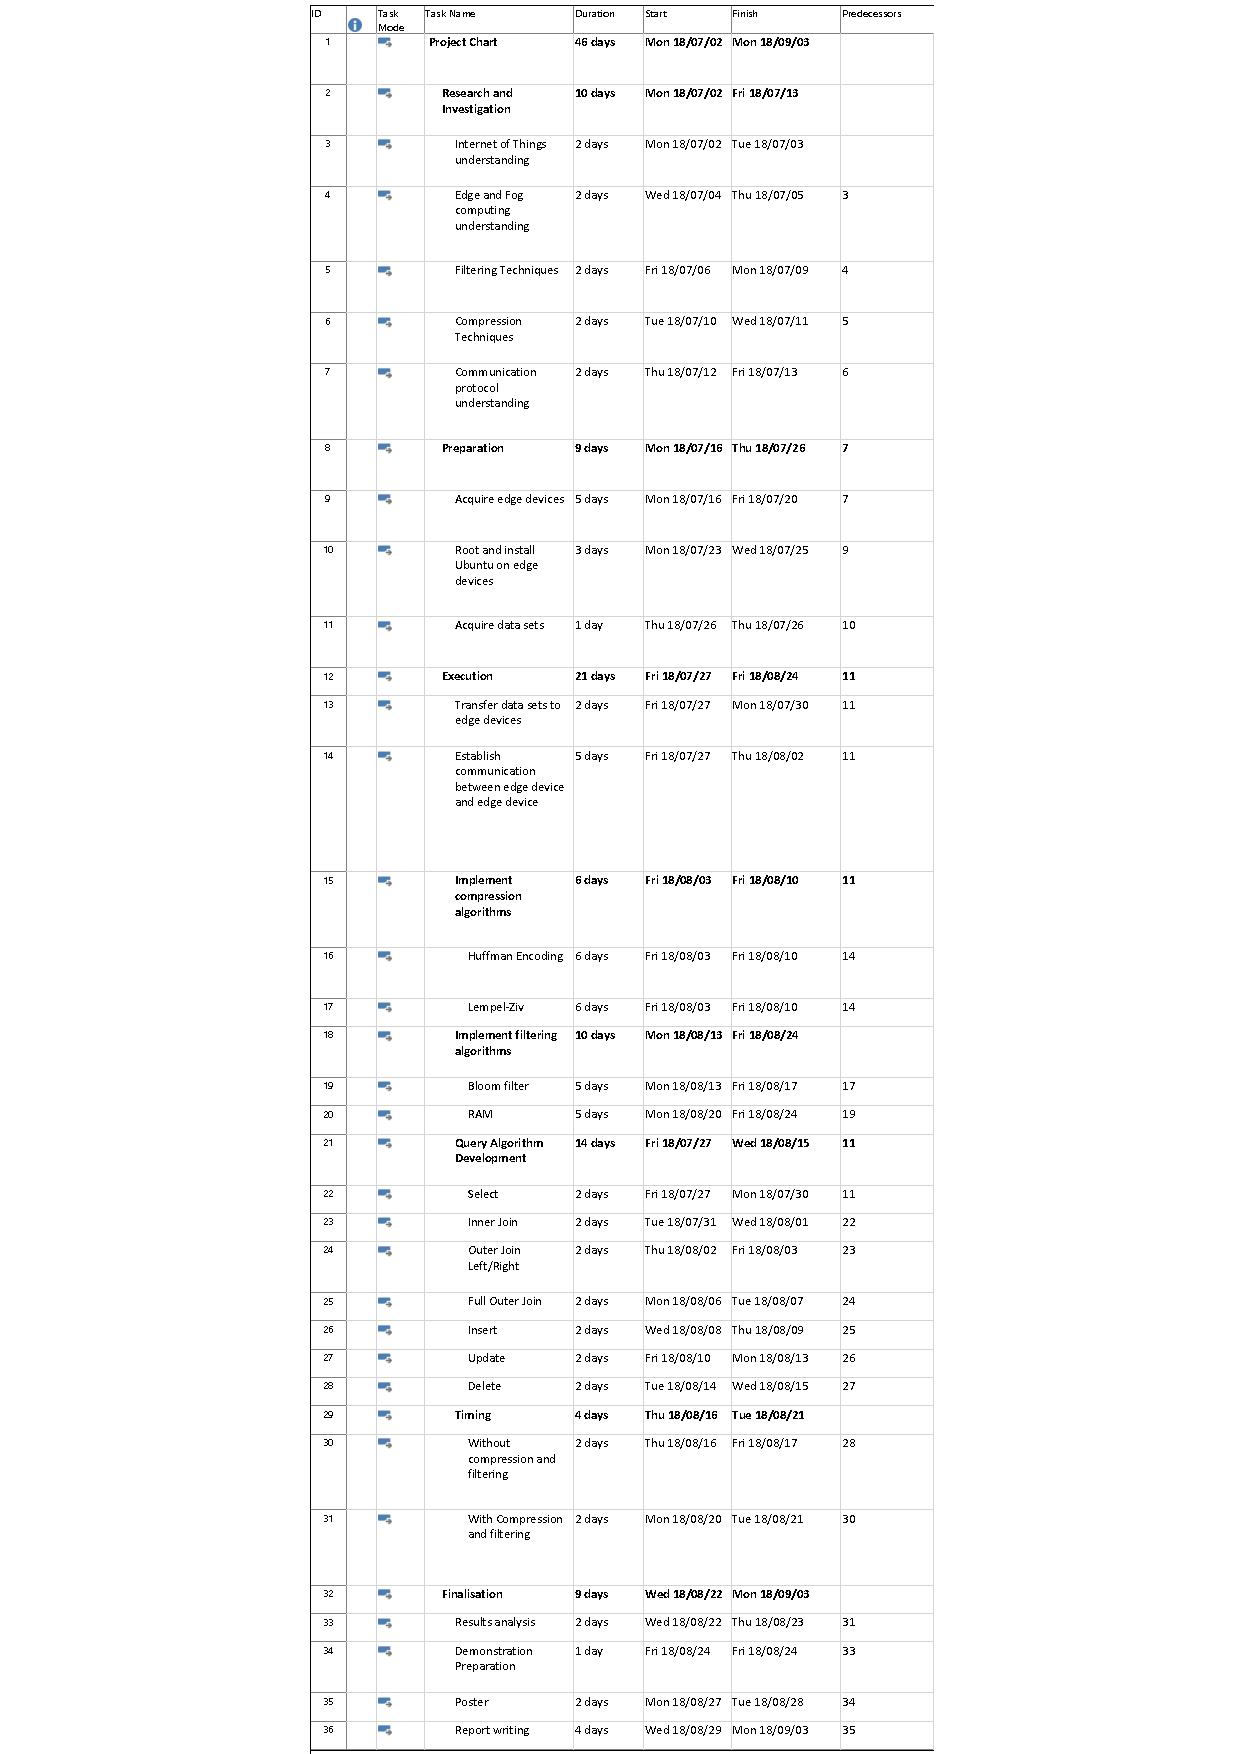
\includegraphics[scale = 0.8]{WBSPROJECT}
\caption{Work Breakdown Structure}
\end{figure}
\end{center}


	% If you have questions about how to write mathematical formulas in LaTeX, please read a LaTeX book or the 'Not So Short Introduction to LaTeX': tobi.oetiker.ch/lshort/lshort.pdf

% Now we need a bibliography:


% Your document ends here!
\end{document}\documentclass[11pt,journal, a4paper]{IEEEtran}
